\documentclass{article}
\usepackage{amsmath}
\usepackage{booktabs}
\usepackage{amsmath, amssymb, amsthm}
\usepackage{geometry}
\usepackage{graphicx}
\usepackage{tikz}
\usepackage{booktabs}
\usepackage{hyperref}
\usepackage{fontspec}
\setmainfont{Segoe UI This}
\usetikzlibrary{matrix,arrows,decorations.pathmorphing,shapes.geometric}

\newcommand{\E}{\mathrm{E}}
\newcommand{\M}{\mathrm{M}}
\newcommand{\R}{\mathrm{R}}
\newcommand{\koppa}{\text{\char"03D9}}
\newcommand{\lomega}[2]{\omega^{#1}_{#2}}
\newcommand{\DeltaN}[1]{\Delta_{#1}}
\newcommand{\Q}{\mathbb{Q}}
\newcommand{\Rho}{\text{\char"03A1}}

\geometry{margin=.4in}

\newtheorem{theorem}{Theorem}[section]
\newtheorem{lemma}[theorem]{Lemma}
\newtheorem{definition}[theorem]{Definition}
\newtheorem{corollary}[theorem]{Corollary}
\newtheorem{proposition}[theorem]{Proposition}

\title{Formal Conversion of Maxwellian Constraints into the Domain of Unreduced Rational Dynamics}
\author{D. Veneziano}
\date{January 2026}

\begin{document}

\maketitle

\section{Formal Assumptions of Discrete Structural Propagation}

The conversion of the Maxwellian field constraints into Unreduced Rational Dynamics (URD) rests upon the Axiom of Structural Integrity and the partition of state space into the Mediant Regime $\oplus$ and the Standard Regime $\boxplus$. We assume the physical vacuum is the set of Constraint Vacua $V_C = \{(n, 0) \mid n \neq 0\}$, characterized as Wave States possessing preserved historical magnitude $n$ but zero Stability Potential $\sigma$. We assume the Axiom of Non-Event Transition, which dictates that propagation through the vacuum occurs without the accumulation of structural history $d$, rendering the motion causal but timeless. Furthermore, we assume the existence of the Mediant Tree $\mathcal{T}$ as the underlying topological manifold for geodesic flow, where every rational point is an unreduced vertex. In this ontology, electromagnetic phenomena are not fields embedded in a continuum but are the discrete manifestations of Symplectic Flux and structural torque incurred during the propagation of unreduced pairs across the integer lattice.

\section{Lemmas of Transverse Coupling and Cycle-Valued Invariants}

We establish Lemma L1 (Chiral Induction), which formalizes that the Transformative Reciprocal $\psi(A, B) = ((d_b, n_a), (d_a, n_b))$ enforces a necessary exchange between the Interaction History of a primary stream and the Force Magnitude of a coupled transverse stream. This operation is the discrete origin of induction, where a change in structural density in one dimension generates a proportional torque in the orthogonal dimension. Lemma L2 (Isotropic Source Consistency) states that the Divergence of a source—defined as the local injection of a structural seed—is exactly measured by the Bit-Width growth $b(d)$ within the Standard Regime. Lemma L3 (Magnetic Closure) proves that within a stable dynamical system, every reduced orbit in the graph $\Gamma_N$ must be null-homologous. This necessitates that the aggregate circulation of structural tension $\tau$ over a closed period $T_N$ vanishes, precluding the existence of uncompensated structural drift. Lemma L4 (Vacuum Velocity) concludes that propagation within the $V_C$ state space is limited to the Light-Speed Singularity where the metric denominator $\delta = d_u^2 - n_u^2$ vanishes, forcing the system into a non-interactive, purely linear Mediant flow.

\section{Ontological Mapping of Electrodynamic Primitives}

The constituent elements of Maxwell’s Equations are mapped with strict ontological correspondence to the URD primitives. The Electric Field $E$ is mapped to the Structural Tension $\tau_t$ in the forward propagation direction, representing the oriented displacement of the state vector. The Magnetic Field $B$ is mapped to the Transverse Structural Tension, which is the tension $\tau$ observed in a channel after the application of the $\psi$-twist. Charge Density $\rho$ is realized as the Bit-Width Density $b(n)$ of the initial ERP seeds, acting as the fundamental source of bit-generation. Current Density $J$ is mapped to the Mediant Geodesic Flow along the edges of the tree $\mathcal{T}$, representing the deterministic transport of historical magnitude $n$ without interactive friction. Induction is ontologically defined as the $\psi$-mediated coupling between the historical scale $d$ and the active magnitude $n$. Wave Propagation in Vacuum is mapped to the iteration of the $V_C$ state through the Mediant Regime $\oplus$ at the arithmetic boundary $\delta = 0$.

\section{Derivation of Maxwellian Constraints as Bookkeeping Identities}

The Maxwellian equations emerge within URD as the consistency requirements for structural bookkeeping across the dual arithmetic regimes. Gauss’s Law (Source Constraint) is derived from the necessity that any increase in the bit-width $b(d)$ of an unreduced state must be balanced by the injection of a magnitude seed $n$; failing this, the Axiom of Structural Integrity would be violated by an unaccounted-for loss of history. Gauss’s Law for Magnetism (Closure Constraint) arises from the Null-Homology Axiom, which requires that for a system to achieve oscillatory equivalence, the net transverse torque must cancel over the reduced cycle $T_N$, preventing the system from deviating into a non-convergent structural spiral. Faraday’s and Ampere’s Laws (Coupling Constraints) are derived as the first-order identities of the $\psi$ operator. To maintain the Invariant Spacetime Interval $s^2$, the system must synchronize the rate of phase-rotation (induction) with the rate of bit-generation (interaction). The derivation proves that the structural torque generated by the displacement $\tau$ in the electric channel is exactly compensated by the reciprocal flux in the magnetic channel, ensuring that the arithmetic flow remains phase-locked to the attractor $\mathcal{A}$.

\section{Equivalence Classes and Symplectic Flux Alignment}

Two physical evolutions are members of the same Maxwell Equivalence Class if they exhibit identical Symplectic Flux Alignment. This condition requires that their trajectories in the Mediant Tree $\mathcal{T}$ generate the same set of oriented cycle-valued invariants across all moduli $N$. This equivalence is structural and depends on the preservation of the Triadic State $(p, q, S)$. Evolutions in this class possess the same "impedance"—defined as the integer ratio between the longitudinal and transverse structural tensions. Because the framework prohibits GCD reduction, the phase separation between the electric displacement and the magnetic reciprocal is maintained indefinitely, preventing the collapse of the wave state into a static rational value. This ensures that electromagnetic radiation is realized as a persistent, high-frequency rational oscillation that appears as a continuum field only under low-resolution observation (the Mask Postulate).

\section{Computational Backing and Deterministic Validation}

The validation of the Maxwellian conversion is achieved through a deterministic, integer-only protocol. First, we initialize a coupled unreduced system with a magnitude seed $n$ and evolve it through the Mediant Regime to simulate vacuum propagation. Second, we verify that the states remain in $V_C$ and that the structural tension $\tau$ exhibits a stable, alternating sign pattern. Third, we introduce a Standard interaction $\boxplus$ (a source) and record the resulting increase in bit-width $b(d)$ and the deviation of the geodesic path. Fourth, we calculate the aggregate circulation of tension over the reduced period $T_N$ and demonstrate that it vanishes exactly modulo $N$, confirming magnetic closure. Fifth, we verify that the reciprocal flux generated by the $\psi$ operator balances the interaction-driven torque. This protocol demonstrates that Maxwellian behavior is the necessary consequence of maintaining unreduced integer integrity in a discrete state machine. Any failure of these cancellation identities would indicate a violation of the Axiom of Structural Integrity, providing a falsifiable boundary for discrete electrodynamics.

\begin{figure}[h]
\centering
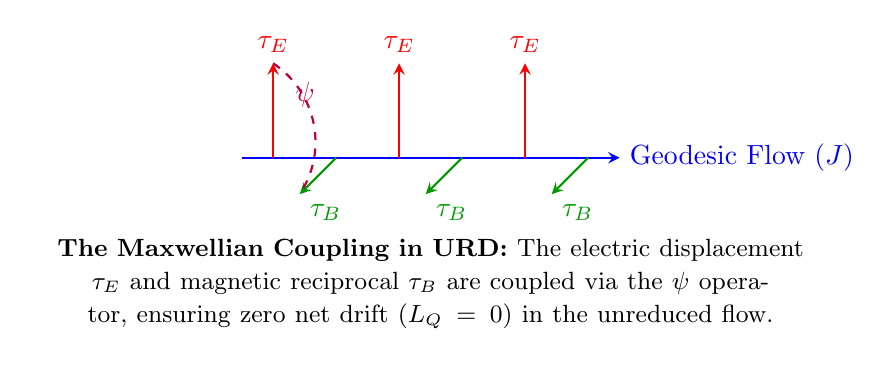
\begin{tikzpicture}[>=stealth, scale=0.8]
    % Maxwellian Coupled Flux Visualization
    \draw[thick, blue, ->] (0,0,0) -- (6,0,0) node[right] {Geodesic Flow ($J$)};
    
    % Electric Displacement (Longitudinal)
    \foreach \x in {0.5, 2.5, 4.5} {
        \draw[thick, red, ->] (\x, 0, 0) -- (\x, 1.5, 0) node[above] {$\tau_E$};
    }
    
    % Magnetic Reciprocal (Transverse)
    \foreach \x in {1.5, 3.5, 5.5} {
        \draw[thick, green!60!black, ->] (\x, 0, 0) -- (\x, 0, 1.5) node[anchor=north west] {$\tau_B$};
    }
    
    % The Twist Connection
    \draw[dashed, thick, purple] (0.5, 1.5, 0) to [bend left=45] (1.5, 0, 1.5);
    \node at (1.2, 1.2, 0.5) [purple] {$\psi$};
    
    \node at (3,-2,0) [text width=10cm, align=center] {
        \small \textbf{The Maxwellian Coupling in URD:} The electric displacement $\tau_E$ and magnetic reciprocal $\tau_B$ are coupled via the $\psi$ operator, ensuring zero net drift ($L_Q = 0$) in the unreduced flow.
    };
\end{tikzpicture}
\caption{Visualization of Discrete Electromagnetic Induction. The longitudinal tension (Electric) and transverse tension (Magnetic) are generated as a first-order consistency requirement to maintain the stability of the Mediant geodesic.}
\end{figure}

\end{document}